\documentclass[a4paper, addpoints]{exam}

\usepackage{amsfonts,amsmath,amsthm}
\usepackage[a4paper]{geometry}
\usepackage{tikz}
\usetikzlibrary{positioning}

\tikzset{
    square/.pic={
      \node[draw, minimum size=40pt, thick] (a) {};
      \draw[dashed] (a.north) -- (a.south);
      \draw[dashed] (a.east) -- (a.west);
    }}

\tikzset{
    tall/.pic={
      \node[draw, minimum height=40pt, minimum width=20pt, thick] (a) {};
      \draw[dashed] (a.east) -- (a.west);
    }}

\tikzset{
    wide/.pic={
      \node[draw, minimum width=40pt, minimum height=20pt, thick] (a) {};
      \draw[dashed] (a.north) -- (a.south);
    }}

\header{CS/MATH 113}{WC12: Strong Induction}{Spring 2024}
\footer{}{Page \thepage\ of \numpages}{}
\runningheadrule
\runningfootrule

\printanswers

\qformat{{\large\bf \thequestion. \thequestiontitle}\hfill}
\boxedpoints

\title{Weekly Challenge 12: Strong Induction}
\author{CS/MATH 113 Discrete Mathematics}
\date{Spring 2024}

\begin{document}
\maketitle

\begin{questions}
  \titledquestion{Stax}
    The game of \textit{Stax} is played with an abundant supply of tiles of 3 different types, shown below.
    \begin{center}
    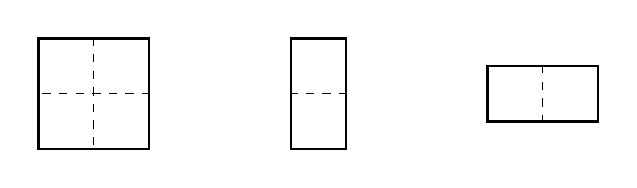
\begin{tikzpicture}
      \matrix (A) [column sep=50pt] {
        \pic{square}; & \pic{tall}; & \pic{wide};\\
      };
    \end{tikzpicture}
  \end{center}
  
  The objective is to completely tile a $n\times 2$ board using the available tiles. 5 different tilings of a $4\times 2$ board are shown below.
    \begin{center}
    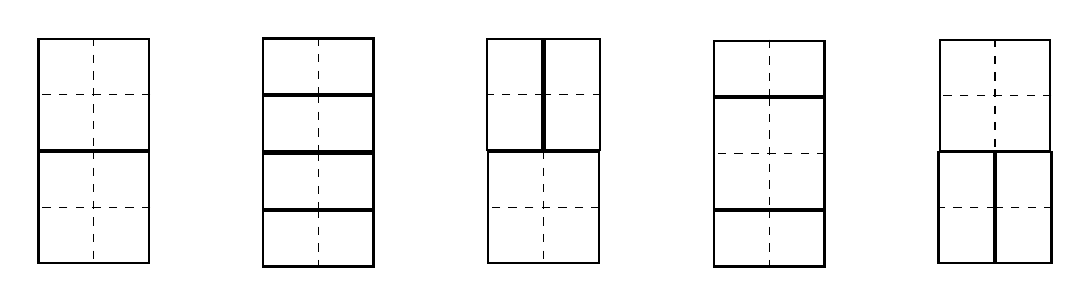
\begin{tikzpicture}
      \matrix (A) [column sep=40pt] {
      \pic [local bounding box = a] at (0,0) {square};
      \pic [above = 0pt of a, local bounding box = b] {square}; &
      \pic [local bounding box = c] at (0,-0.4) {wide};
      \pic [above = 0pt of c, local bounding box = d] {wide};
      \pic [above = 0pt of d, local bounding box = e] {wide};
      \pic [above = 0pt of e, local bounding box = f] {wide};&
      \pic [local bounding box = g] at (0,0) {square};
      \pic [above = 0pt of g, anchor = south east, local bounding box = h] {tall};
      \pic [right = 0pt of h, local bounding box = i] {tall};&
      \pic [local bounding box = j] at (0,-0.4) {wide};
      \pic [above = 0pt of j, local bounding box = k] {square};
      \pic [above = 0pt of k, local bounding box = l] {wide};&
      \pic [local bounding box = m] at (0,0) {tall};
      \pic [right = 0pt of m, local bounding box = n] {tall};
      \pic [above = 0pt of n.north west, local bounding box = o] {square};\\
    };
    \end{tikzpicture}
  \end{center}

  Let $T_n$ denote the number of all possible tilings of a $n\times 2$ board.

  \begin{parts}
  \part[2] What are the values of $T_1, T_2,$ and $T_3$?
    \begin{solution}
      % Enter your solution here.
    \end{solution}

  \part[3] Argue why $T_n = T_{n-1} + 2T_{n-2}$.
    \begin{solution}
      % Enter your solution here.
    \end{solution}

  \part[5] Show using strong induction that
    \[
      T_n = \frac{2^{n+1}+(-1)^n}{3}
    \]
    \begin{solution}
      % Enter your solution here.
    \end{solution}
  \end{parts}
\end{questions}

\end{document}
%%% Local Variables:
%%% mode: latex
%%% TeX-master: t
%%% End:
